\documentclass[hyperref=unicode]{beamer}

\usepackage[absolute,overlay]{textpos}
\usepackage{graphicx}
\usepackage{adjustbox}
\usepackage{chemfig}
\usepackage[version=4]{mhchem}
\usepackage{wrapfig}
\usepackage{multirow}
\adjustboxset*{center}
\usepackage{caption}
\usepackage{chemformula}
\usepackage{elements}

%dělení slov
\usepackage{ragged2e}
\let\raggedright=\RaggedRight
%konec dělení slov

\usepackage{fontspec}
\usepackage{unicode-math}

\usepackage{polyglossia}
\setdefaultlanguage{czech}

\def\uv#1{„#1“}

\mode<presentation>{\usetheme{Madrid}}
\DefineNamedColor{named}{pozadi}{RGB}{200,200,200}
\usecolortheme{crane}

\setbeamertemplate{footline}[frame number]

\addtobeamertemplate{frametitle}{
	\let\insertframetitle\insertsectionhead}{}
\addtobeamertemplate{frametitle}{
	\let\insertframesubtitle\insertsubsectionhead}{}

\makeatletter
\CheckCommand*\beamer@checkframetitle{\@ifnextchar\bgroup\beamer@inlineframetitle{}}
\renewcommand*\beamer@checkframetitle{\global\let\beamer@frametitle\relax\@ifnextchar\bgroup\beamer@inlineframetitle{}}
\makeatother
\setbeamercolor{section in toc}{fg=blue}
\setbeamertemplate{section in toc shaded}[default][100]

\usepackage{tikz}
\usetikzlibrary{positioning}
\usetikzlibrary{arrows}
\usetikzlibrary{shapes.multipart}

\title[Crisis]
{Elektrochemie}

\subtitle{Galvanické články, elektrolýza, elektrodový potenciál}

\author{Zdeněk Moravec, hugo@chemi.muni.cz \\ 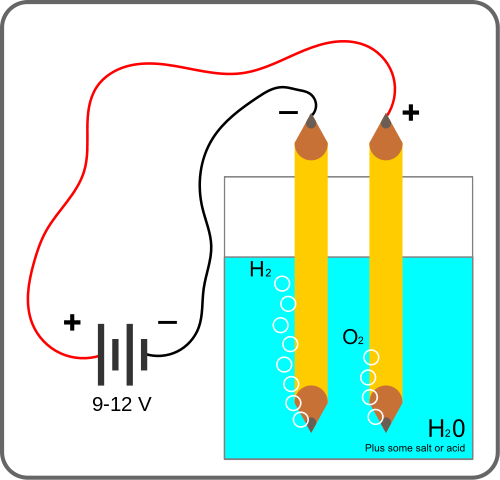
\includegraphics[keepaspectratio,width=4.8cm]{electrolysis.png}}

\begin{document}

\frame{\titlepage}

\section{Elektrodový potenciál}
\frame{
	\frametitle{}
	\vfill
	\begin{itemize}
		\item Elektroda - elektrický vodič ponořený do roztoku elektrolytu
		\begin{itemize}
			\item Elektroda prvního druhu - kov ponořený do roztoku své soli Cu$|$Cu$^{2+}$
			\item Elektroda druhého druhu - kov pokrytý vrstvou jeho nerozpustné sloučeniny ponořený do roztoku rozpustné soli Ag$|$AgCl$|$KCl
		\end{itemize}
		\item Elektrodový potenciál ($E$) - potenciál elektrody vůči standardní vodíkové elektrodě, jednotkou je volt [V]
		\item Standardní elektrodový potenciál ($E^0$) - elektrodový potenciál za standardních podmínek (0~$^\circ$C; 100~kPa)
		\item \textbf{Nernstova rovnice:}
		\item $E = E^0 - \frac{RT}{zF}\ln c = E^0 + \frac{0,0592}{z}\log c$
		\item \textbf{Nernstova-Petersonova rovnice:}
		\item $E = E^0 - \frac{RT}{zF}\ln\frac{a_{red}}{a_{ox}} = E^0 + \frac{0,0592}{z}\log\frac{a_{red}}{a_{ox}}$
	\end{itemize}
	\vfill
}

\frame{
	\frametitle{}
	\begin{columns}

		\column{.4\textwidth}
		\begin{tabular}{|l|r@{,}l|}
			\hline
			\textbf{Elektroda} & \multicolumn{2}{|c|}{\textbf{E$^0$ [V]}} \\\hline
			Li/Li$^+$ & -3 & 045 \\\hline
			Cs/Cs$^+$ & -2 & 923 \\\hline
			Na/Na$^+$ & -2 & 714 \\\hline
			Mg/Mg$^{2+}$ & -2 & 363 \\\hline
			Zn/Zn$^{2+}$ & -0 & 762 \\\hline
			Fe/Fe$^{2+}$ & -0 & 440 \\\hline
			Ni/Ni$^{2+}$ & -0 & 250 \\\hline
			H/H$^+$ & 0 & 000 \\\hline
			Cu/Cu$^{2+}$ & 0 & 337 \\\hline
			Cu/Cu$^+$ & 0 & 521 \\\hline
			Ag/Ag$^+$ & 0 & 799 \\\hline
			Pt/Pt$^{2+}$ & 1 & 200 \\\hline
			Au/Au$^{3+}$ & 1 & 498 \\\hline
			Mn$^{3+}$/Mn$^{2+}$ & 1 & 51 \\\hline
			Ce$^{4+}$/Ce$^{3+}$ & 1 & 61 \\\hline
		\end{tabular}

		\column{.6\textwidth}
		\begin{itemize}
			\item Standardní vodíková elektroda (SVE) - platinový drátek pokrytý platinovou černí, sycený plynným vodíkem pod tlakem 101 325 Pa za teploty 273,15 K, ponořený do roztoku o jednotkové aktivitě H$^+$. Tato elektroda má nulový elektrodový potenciál.
		\end{itemize}
		\begin{figure}
			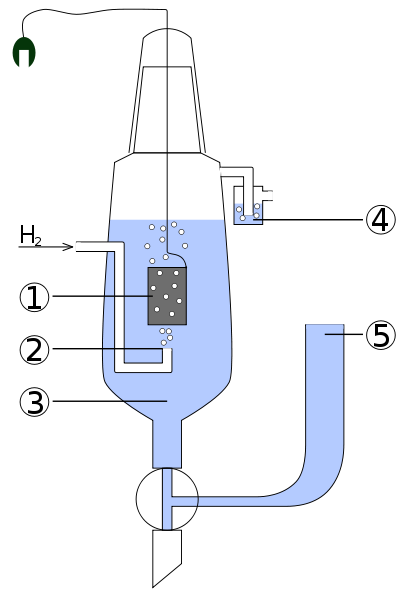
\includegraphics[keepaspectratio,width=3cm]{SVE.png}
		\end{figure}
	\end{columns}
}

\frame{
	\frametitle{}
	\begin{columns}
		\begin{column}{.65\textwidth}
			\begin{itemize}
		\item Čím má kov negativnější potenciál, tím se snadněji oxiduje a má silnější redukční schopnosti.
		\item Cu/Cu$^{2+}$: 0,337 V
		\item Fe/Fe$^{2+}$: $-$0,440 V
		\item \ce{Cu + FeSO4 -> CuSO4 + Fe}
		\begin{itemize}
			\item Měd má kladnější potenciál a proto reakce \textit{nepoběží samovolně}.
		\end{itemize}
		\item \ce{Fe + CuSO4 -> FeSO4 + Cu}
		\begin{itemize}
			\item Železo má zápornější potenciál a proto reakce \textit{poběží samovolně}.
			\item Železný drát ponořený do roztoku modré skalice se po chvíli začne pokrývat vyloučenou mědí.
		\end{itemize}
	\end{itemize}
		\end{column}
	\begin{column}{.35\textwidth}
		\begin{figure}
			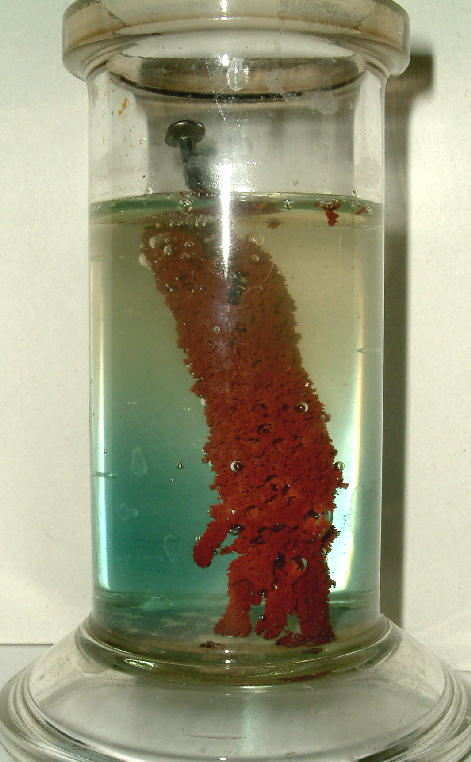
\includegraphics[keepaspectratio,width=\textwidth]{Fe-nagel_in_CuSO4.jpg}
		\end{figure}
	\end{column}
	\end{columns}
}

\section{Galvanický článek}
\frame{
	\frametitle{}
	\vfill
	\begin{itemize}
		\item Chemický zdroj elektrického napětí.
		\item Skládá se ze dvou poločlánků, elektrod ponořených do elektrolytu.
	\end{itemize}
	\begin{figure}
		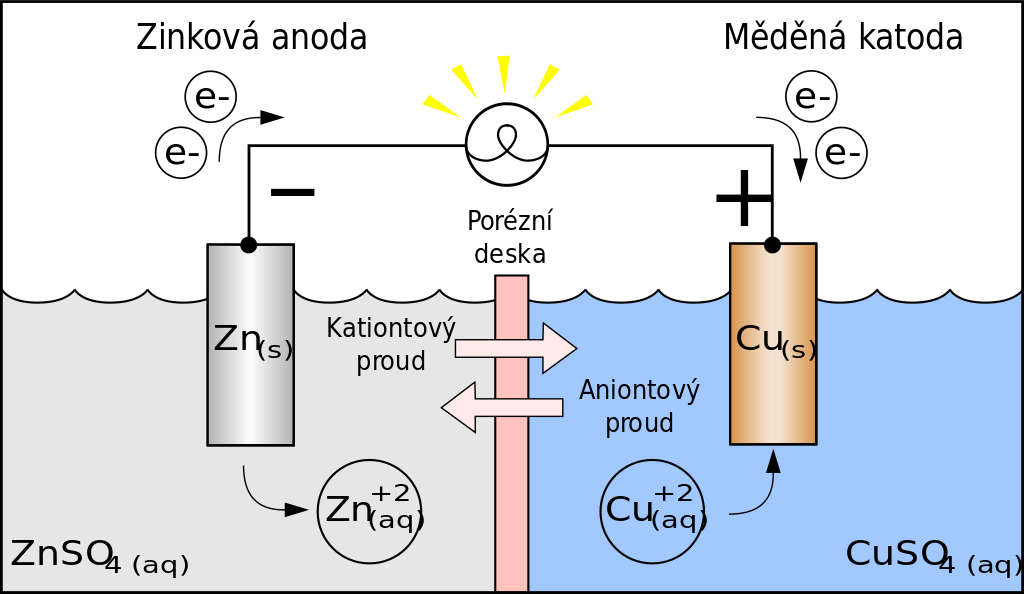
\includegraphics[keepaspectratio,width=.8\textwidth]{Galvanicky_clanek.png}
	\end{figure}
	\vfill
}

\section{Elektrolýza}
\subsection{1. Faradayův zákon}
\frame{
	\frametitle{}
	\vfill
	\begin{itemize}
	\item Probíhá v roztocích nebo taveninách
	\item Elektrolýze může podléhat rozpouštědlo nebo ionty elektrolytu
	\item \ce{2 H2O -> 2 H2 + O2}
	\item \textbf{1. Faradayův zákon}
	\item Hmotnost vyloučené látky je úměrná proudu, který prochází elektrolytem a času, po který elektrolýza probíhala
	\item $m = A.I.t = A.Q$
	\begin{itemize}
	\item A - elektrochemický ekvivalent, I - proud, t - čas, Q - náboj
	\end{itemize}
	\end{itemize}
	\vfill
}

\subsection{2. Faradayův zákon}
\frame{
	\frametitle{}
	\vfill
	\begin{itemize}
	\item \textbf{2. Faradayův zákon}
	\item Látková množství vyloučená jednotkovým nábojem jsou pro všechny látky ekvivalentní.
	\item $A = \frac{M}{Fz}$
	\begin{itemize}
	\item z - počet vyměňovaných elektronů
	\item F - Faradayova konstanta (96 485,33 C.mol$^{-1}$)
	\end{itemize}
	\item Faradayova konstanta odpovídá náboji jednoho molu elektronů.
	\item $F = e.N_A = 1,602 176 565\times 10^{-19} . 6,022 141 29\times 10^{23}$
	\item $F = 96 485,33\ C.mol^{-1}$
	\end{itemize}
	\vfill
}

\subsection{Výpočty}
\frame{
	\frametitle{}
	\vfill
	\begin{itemize}
	\item \emph{Vypočítejte elektrodový potenciál zinkové elektrody, koncentrace elektrolytu je 0,5~mol.dm$^{-3}$ a teplota 25 $^\circ$C.}
	\item Při elektrodovém ději se vyměňují dva elektrony: \ce{Zn -> Zn^{2+}}.
	\item Standardní elektrodový potenciál ($E^0$) Zn/Zn$^{2+}$ je -0,762~V.
	\item $E = E^0 - \frac{RT}{zF}\ln c = -0,762 + \frac{8,314\ .\ 298,15}{2\ .\ 96 485,33} ln(0,5) = -0,771~V$
	\end{itemize}
	\hrulefill
	\begin{itemize}
	\item \emph{Vypočítejte potenciál platinového drátku ponořeného do roztoku, kde je koncentrace Fe$^{2+}$ 0,15~mol.dm$^{-3}$ a koncentrace iontů Fe$^{3+}$ 0,05~mol.dm$^{-3}$, měření probíhá za teploty 0~$^\circ$C.}
	\item Při elektrodovém ději se vyměňuje jeden elektron: \ce{Fe^{2+} -> Fe^{3+}}.
	\item Standardní elektrodový potenciál ($E^0$) Fe$^{3+}$/Fe$^{2+}$ je 0,771~V.
	\item $E = E^0 - \frac{RT}{zF}\ln (\frac{[red]}{[ox]}) = 0,771 - \frac{8,314\ .\ 273,15}{1\ .\ 96 485,33} ln(\frac{0,15}{0,05}) = 0,745~V$
	\end{itemize}
	\vfill
}

\iffalse
\section{Další informace}
\frame{
	\frametitle{}

	\href{http://z-moravec.net/chemie/zaklady-chemie/}{http://z-moravec.net/}
}
\fi

\end{document}